% Provenance (never printed): see sources/outline_sources.md (Year 3:
% planetary atmospheres, escape, the runaway greenhouse, Mars, Titan,
% habitability).
% Brief: sources/book5/BRIEFS.md, ch. 27. Curves from figdata/bachelor-3/
% jeans_escape.py (escape parameter and escaping fraction at the exobases
% of Venus, the Earth, Mars and Titan), runaway_greenhouse.py (an
% illustrative grey model of a moist atmosphere: OLR against surface
% temperature) and habitability.py (the habitable-zone fits of Kopparapu et
% al. 2013; the phase boundaries of water and methane with the surface
% states of four bodies). Exercise and problem values in the Book 5 scratch
% calculator calc/ch27.py. Kepos and its star are invented.
\chapter{ग्रहीय वायुमंडल और वासयोग्यता}\label{ch:b3:planetary-atmospheres}

शुक्र और पृथ्वी लगभग जुड़वाँ हैं: आकार लगभग समान, मिलते-जुलते माध्य
घनत्व, पड़ोसी कक्षाएँ। फिर भी शुक्र \qty{92}{bar} कार्बन डाइऑक्साइड बनाए रखता है,
जो \qty{737}{K} तापमान वाली सतह के ऊपर है, और पानी इतना कम कि
उसे सतह पर फैलाएँ तो लगभग एक सेंटीमीटर गहरी परत बने। पायनियर वीनस यान के
द्रव्यमान स्पेक्ट्रममापी ने, बादलों से होकर गिरते हुए, उस पानी में
ड्यूटेरियम और हाइड्रोजन का अनुपात मापा: \num{0.016},
जो पृथ्वी के महासागरों के अनुपात का सौ गुना है। हल्का हाइड्रोजन
भारी ड्यूटेरियम की तुलना में अंतरिक्ष में अधिक आसानी से निकल जाता है; बड़े भंडार का जो शेष है,
जिसने अपना अधिकांश हाइड्रोजन खो दिया है, वह ड्यूटेरियम से समृद्ध होता है। यह अनुपात उस पानी का चिह्न है
जो शुक्र पर कभी था और खो गया। यह अध्याय पूछता है कि कोई ग्रह
अपनी हवा और पानी को कैसे थामे रखता है, और उन्हें कैसे खोता है।
% ledger: planet:Venus.diameter, planet:Earth.diameter, planet:Venus.density, planet:Earth.density, nasa:venus-atm, arney18:venus-water, donahue82:dh, kc98:standards

\begin{recall}
स्केल ऊँचाई, वायुदाब सूत्र, मैक्सवेल--बोल्ट्ज़मान
वितरण, पलायन वेग, माध्य मुक्त पथ और हरितगृह
प्रभाव भौतिकी की पुस्तकों में हैं। किसी तारे का वासयोग्य क्षेत्र
विद्यालय की पुस्तकों में है। साम्य तापमान और बॉन्ड एल्बिडो
पुस्तक 3 (स्नातक वर्ष 1) में हैं, तुलनात्मक ग्रहविज्ञान वाले अध्याय में; प्रकाशीय गहराई
दूरदर्शी और प्रकाशमिति वाले अध्याय में; तापह्रास दरें वायुमंडल
और महासागर की संरचना वाले अध्याय में; बाह्य दीर्घ-तरंग विकिरण
(OLR) और उत्सर्जन तापमान, विकिरण और ऊष्मा परिवहन वाले अध्याय में।
आर्द्र रुद्धोष्म वक्र पुस्तक 4 (स्नातक वर्ष 2) में है,
वायुमंडलीय ऊष्मागतिकी वाले अध्याय में; हिम रेखा ग्रह-निर्माण वाले
अध्याय में; दीर्घकालिक कार्बन चक्र और सिलिकेट-अपक्षय तापस्थापी
भूवैज्ञानिक समय की जलवायु वाले अध्याय में। \omterm{prop:b3:stable-isotopes:rayleigh-distillation}{रैले आसवन} इसी पुस्तक में है,
स्थिर
समस्थानिक वाले अध्याय में।
\end{recall}

\section{वायुमंडल की संरचना}\label{sec:b3:planetary-atmospheres:structure}

आणविक द्रव्यमान $m$ और तापमान $T$ वाला समतापी वायुमंडल, ऊँचाई के साथ दाब
$p = p_0\,e^{-z/H}$ के रूप में घटता है, जहाँ स्केल ऊँचाई $H = kT/mg$ है।
पृथ्वी की सतह पर $H$ लगभग \qty{8}{km} है; टाइटन की सतह पर
जहाँ गुरुत्व दुर्बल और वायु ठंडी है, वह लगभग \qty{20}{km} है।

तापमान, हालाँकि, एक-समान नहीं है। भूतल तक पहुँचने वाला सूर्य का प्रकाश
उसे गर्म करता है; ऊपर की वायु, जो अवरक्त में अवशोषण और उत्सर्जन करती है,
नीचे से गर्म होती है। केवल विकिरण से निचला वायुमंडल
तापमान में इतना तीव्र ढाल वाला हो जाता कि वह उलट पड़ता।

\begin{definition}[विकिरणी--संवहनी साम्य]\label{def:b3:planetary-atmospheres:rce}
वायुमंडल का एक स्तंभ \emph{विकिरणी--संवहनी
साम्य}\index{विकिरणी--संवहनी साम्य} में होता है, जब हर स्तर पर
विकिरण का शुद्ध फ़्लक्स संतुलित होता है, सिवाय उस निचली परत के
जहाँ संवहन ऊष्मा को ऊपर ले जाता है और तापमान-प्रवणता को
रुद्धोष्म प्रवणता पर रखता है। निचली, संवहनी परत क्षोभमंडल है; ऊपरी
परत, जो विकिरणी साम्य में है, समतापमंडल; क्षोभसीमा
वह स्तर है जहाँ वे मिलते हैं।
\end{definition}

इसका अनुसरण जिस सबसे सरल वायुमंडल में किया जा सकता है, वह \emph{धूसर} है: वह
सूर्य के प्रकाश के लिए पारदर्शी है, और हर अवरक्त तरंगदैर्घ्य को समान रूप से अवशोषित करता है,
जिसकी प्रकाशीय गहराई $\tau$ ऊपर से नीचे की ओर गिनी जाती है।

\begin{proposition}[धूसर विकिरणी साम्य]\label{prop:b3:planetary-atmospheres:grey}
विकिरणी साम्य में एक धूसर वायुमंडल, जो अंतरिक्ष की ओर फ़्लक्स $F$ उत्सर्जित करता है,
प्रकाशीय गहराई $\tau$ पर तापमान इस संबंध का पालन करता है:
\[
\sigma T^4(\tau) = \frac F2\,(1 + D\tau),
\]
जहाँ $D \approx 1.66$ विकिरण के तिरछे पथों का हिसाब रखता है।
वायुमंडल का शीर्ष \emph{त्वचा तापमान} पर होता है,
जो $T_\text{त्वचा} = 2^{-1/4}\,T_e$ के बराबर है, जहाँ $T_e = (F/\sigma)^{1/4}$
उत्सर्जन तापमान है।
\end{proposition}

यह प्रतिज्ञप्ति मान ली गई है; यह ऊपर और नीचे की ओर के फ़्लक्स के लिए
दो-धारा समीकरणों से निकलती है। जहाँ $\tau$ बड़ा है, भूतल के पास,
विकिरणी तापमान $\tau$ के साथ तेज़ी से बदलता है, और $\tau$ स्वयं
गहराई के साथ तेज़ी से बढ़ता है, क्योंकि अवशोषक गैस वहाँ सबसे घनी है:
विकिरणी प्रोफ़ाइल रुद्धोष्म वक्र से अधिक तीव्र है, और संवहन कार्यभार संभाल लेता है।
ऊपर की ओर $\tau$ छोटा है और तापमान त्वचा तापमान की ओर जाता है। पृथ्वी
अंतरिक्ष की ओर लगभग \qty{239}{W.m^{-2}} उत्सर्जित करती है, उत्सर्जन तापमान
\qty{255}{K} और त्वचा तापमान \qty{214}{K} है; मानक वायुमंडल क्षोभसीमा
\qty{11}{km} पर रखता है, वहाँ तापमान
\qty{216.65}{K} है। यह धूसर मॉडल, जितना भी अपरिष्कृत है,
क्षोभमंडल के ठंडे शीर्ष को लगभग सही जगह पर रखता है।
% ledger: ipcc:budget-toa, ussa76:sea-level, ussa76:layers, const:sigma

\begin{omfigure}
\centering
\begin{tikzpicture}[x=1cm, y=0.8cm, font=\small]
% temperature profile (schematic)
\draw[->] (0,0) -- (6.8,0) node[below left, font=\scriptsize] {तापमान};
\draw[->] (0,0) -- (0,8.4) node[above, font=\scriptsize] {ऊँचाई};
\draw[thick, omDef] (5.6,0) -- (4.2,2.0) -- (4.2,2.6) -- (4.7,3.6)
  -- (3.8,4.6) .. controls (4.3,5.6) and (5.9,6.0) .. (6.2,6.6) -- (6.25,8.2);
\draw[dashed, black!50] (0,2.0) -- (6.8,2.0) node[right, font=\scriptsize, black] {क्षोभसीमा};
\draw[dashed, black!50] (0,4.6) -- (6.8,4.6) node[right, font=\scriptsize, black] {होमोपॉज़};
\draw[thick, red!70!black] (0,6.6) -- (6.8,6.6) node[right, font=\scriptsize] {बाह्य-आधार};
\node[anchor=west, font=\scriptsize] at (0.15,0.9) {क्षोभमंडल: संवहन};
\node[anchor=west, font=\scriptsize] at (0.15,0.5) {(रुद्धोष्म)};
\node[anchor=west, font=\scriptsize] at (0.15,3.2) {समतापमंडल:};
\node[anchor=west, font=\scriptsize] at (0.15,2.8) {विकिरणी साम्य};
\node[anchor=west, font=\scriptsize] at (0.15,5.6) {तापमंडल};
\node[anchor=west, font=\scriptsize] at (0.15,5.2) {(EUV द्वारा तप्त)};
\node[anchor=west, font=\scriptsize] at (0.15,7.6) {बाह्यमंडल:};
\node[anchor=west, font=\scriptsize] at (0.15,7.2) {कोई टक्कर नहीं};
% exosphere trajectories
\begin{scope}[shift={(11.0,0)}]
\fill[black!8] (-2.3,0) rectangle (2.3,6.6);
\draw[red!70!black, thick] (-2.3,6.6) -- (2.3,6.6);
\node[font=\scriptsize] at (0,0.5) {हर जगह टक्कर};
\node[font=\scriptsize, align=center] at (0,3.3) {गैस प्रक्षुब्धता से\\मिश्रित, होमोपॉज़ के\\नीचे; आणविक विसरण\\से पृथक होकर\\उसके ऊपर};
\draw[->, thick, omDef] (-1.6,6.6) .. controls (-1.4,8.0) and (-0.9,8.0) .. (-0.7,6.6);
\node[font=\scriptsize, omDef] at (-1.15,8.3) {प्रक्षेपीय};
\draw[->, thick, red!70!black] (0.4,6.6) -- (1.2,8.5);
\node[font=\scriptsize, red!70!black, anchor=west] at (1.25,8.3) {पलायन};
\node[font=\scriptsize, align=center, anchor=north] at (0,6.45) {$v > v_\mathrm{esc}$ ऊपर की ओर:\\ अंतरिक्ष में खोया};
\end{scope}
\end{tikzpicture}
\par\smallskip{\small ग्रहीय वायुमंडल की परतें (योजनाबद्ध,
पैमाने पर नहीं)। बाएँ: पृथ्वी जैसी तापमान प्रोफ़ाइल, जिसमें
क्षोभमंडल संवहन द्वारा रुद्धोष्म वक्र पर रखा गया है, विकिरणी साम्य में एक समतापमंडल,
चरम-पराबैंगनी सौर प्रकाश द्वारा ऊपर से तप्त एक तापमंडल। दाएँ:
\omterm{def:b3:planetary-atmospheres:exobase}{बाह्य-आधार} के ऊपर कोई कण किसी से नहीं टकराता; जो कण ऊपर की ओर
पलायन वेग से तेज़ चलता है, वह ग्रह छोड़ देता है; धीमा कण
प्रक्षेपीय चाप पर वापस गिरता है।}\label{fig:b3:planetary-atmospheres:structure}
\end{omfigure}
% ledger: gronoff:exobase, gronoff:diffusion

वायुमंडल में बहुत ऊपर वायु इतनी विरल होती है कि कोई अणु
दो टकरावों के बीच काफ़ी दूर तक जा सकता है। जहाँ वह एक
पैमाना ऊँचाई से अधिक दूरी तय कर सकता है, वहाँ वह अब द्रव का हिस्सा नहीं रहता।

\begin{definition}[बाह्य-आधार; बाह्यमंडल]\label{def:b3:planetary-atmospheres:exobase}
किसी वायुमंडल का \emph{बाह्य-आधार}\index{बाह्य-आधार} वह स्तर है जिस पर
उसके कणों का माध्य मुक्त पथ पैमाना ऊँचाई के बराबर होता है। इसके ऊपर का
\emph{बाह्यमंडल}\index{बाह्यमंडल} है, जहाँ ऊपर की ओर चलने वाले कण की
किसी दूसरे कण से टक्कर की संभावना कम होती है, और स्थानीय पलायन वेग से
तेज़ चलने वाला कण ग्रह को छोड़ देता है।
\end{definition}

\begin{proposition}[बाह्य-आधार की शर्त]\label{prop:b3:planetary-atmospheres:exobase}
समतापीय वायुमंडल में, जिसके कणों का टक्कर-अनुप्रस्थ काट
$\sigma_c$ है, घनत्व-स्तर $n$ से ऊर्ध्वाधर ऊपर की ओर चलने वाला कण
हर टक्कर से बच निकलने की प्रायिकता $e^{-n\sigma_c H}$ होती है।
\omterm{def:b3:planetary-atmospheres:exobase}{बाह्य-आधार} पर $n\sigma_c H = 1$ होता है, और प्रायिकता $1/e$ है।
\end{proposition}

\begin{proof}
पथ $\mathrm dz$ पर कण औसतन $n(z)\sigma_c\,
\mathrm dz$ अन्य कणों से मिलता है। ऊपर जाते समय किसी से न मिलने की
प्रायिकता $z_0$ पर $\exp(-\sigma_c\int_{z_0}^\infty n\,\mathrm dz)$ है, और समतापीय
वायुमंडल में $\int_{z_0}^\infty n_0\,e^{-(z-z_0)/H}\,\mathrm dz
= n_0 H$ होता है। माध्य मुक्त पथ $\ell = 1/n\sigma_c$ है; शर्त $\ell
= H$ का अर्थ है $n\sigma_c H = 1$।
\end{proof}

\omterm{def:b3:planetary-atmospheres:exobase}{बाह्य-आधार} पृथ्वी पर लगभग \qty{500}{km} पर, शुक्र और मंगल पर
\qty{200}{km} पर, और टाइटन पर लगभग \qty{1500}{km} पर स्थित है, जो
टाइटन की त्रिज्या के आधे से अधिक है।
% ledger: gronoff:exobases

\section{वायुमंडलीय पलायन}\label{sec:b3:planetary-atmospheres:escape}

\omterm{def:b3:planetary-atmospheres:exobase}{बाह्य-आधार} पर कण नीचे की गैस के मैक्सवेल--बोल्ट्ज़मान
चाल-वितरण को बनाए रखते हैं। उसकी पूँछ में सदा कुछ ऐसे कण होते हैं जो
पलायन वेग से तेज़ चलते हैं।

\begin{definition}[जीन्स पलायन; पलायन प्राचल]\label{def:b3:planetary-atmospheres:jeans-escape}
\emph{जीन्स पलायन}\index{जीन्स पलायन} वह अंतरिक्ष में होने वाली हानि है, जो
मैक्सवेल--बोल्ट्ज़मान पूँछ के उन कणों की होती है जो \omterm{def:b3:planetary-atmospheres:exobase}{बाह्य-आधार} पर ऊपर की ओर
पलायन वेग से तेज़ चलते हैं। \emph{पलायन
प्राचल}\index{पलायन प्राचल} \omterm{def:b3:planetary-atmospheres:exobase}{बाह्य-आधार} पर द्रव्यमान $m$ वाले कणों का,
त्रिज्या $r$ और तापमान $T$ वाले, द्रव्यमान $M$ के ग्रह पर, इस प्रकार होता है
\[
\lambda = \frac{GMm}{kTr} = \frac{v_\mathrm{esc}^2}{u^2},
\qquad u = \sqrt{\frac{2kT}m},
\]
यह उनकी गुरुत्वीय बंधन ऊर्जा और $kT$ का अनुपात है, और साथ ही
सबसे संभावित तापीय चाल $u$ पर पलायन वेग के वर्ग का अनुपात भी है।
\end{definition}

\begin{theorem}[जीन्स फ़्लक्स]\label{thm:b3:planetary-atmospheres:jeans}
घनत्व $n$ वाले \omterm{def:b3:planetary-atmospheres:exobase}{बाह्य-आधार} पर, प्रति इकाई क्षेत्रफल और प्रति इकाई
समय पलायन करने वाले कणों की संख्या है
\[
\Phi_\mathrm J = \frac{n\,u}{2\sqrt\pi}\,(1 + \lambda)\,e^{-\lambda}.
\]
\end{theorem}

\begin{proof}
मैक्सवेल--बोल्ट्ज़मान वेग-वितरण $f(\vec v) =
n\,(\pi u^2)^{-3/2}\,e^{-v^2/u^2}$ है। चाल $v$ से चलने वाला कण, जो
ऊर्ध्वाधर से कोण $\theta$ पर चलता है, क्षैतिज इकाई क्षेत्रफल को
दर $v\cos\theta$ से पार करता है। केवल ऊपर की ओर के वेग ($0 \le \theta \le
\pi/2$) गिनते हुए, जो $v_\mathrm{esc}$ से तेज़ हैं,
\[
\Phi_\mathrm J = \frac{n}{\pi^{3/2}u^3}\int_0^{2\pi}\!\!\mathrm d\varphi
\int_0^{\pi/2}\!\!\cos\theta\sin\theta\,\mathrm d\theta
\int_{v_\mathrm{esc}}^\infty v^3e^{-v^2/u^2}\,\mathrm dv
= \frac{n}{\pi^{3/2}u^3}\cdot2\pi\cdot\frac12\cdot
\frac{u^4}2\,(1 + \lambda)\,e^{-\lambda},
\]
जहाँ अंतिम समाकल प्रतिस्थापन $s = v^2/u^2$ से और
एक बार खंडशः समाकलन से निकलता है: $\int_\lambda^\infty s\,e^{-s}\,\mathrm ds =
(1 + \lambda)e^{-\lambda}$। समेटने पर, $\Phi_\mathrm J = n u (1 +
\lambda) e^{-\lambda}/(2\sqrt\pi)$।
\end{proof}

$n u/2\sqrt\pi$ गुणांक \omterm{def:b3:planetary-atmospheres:exobase}{बाह्य-आधार} को ऊपर की ओर पार करने वाले सभी कणों का
फ़्लक्स है, और $(1 + \lambda)e^{-\lambda}$ उनमें से पलायन करने वाला भाग है।
यह कण के द्रव्यमान के साथ घातांकीय रूप से घटता है, क्योंकि
$\lambda \propto m$। पृथ्वी के \omterm{def:b3:planetary-atmospheres:exobase}{बाह्य-आधार} पर, \qty{1000}{K} पर हाइड्रोजन का
$\lambda = 7.0$ है, और वह अपने ऊपर की ओर के फ़्लक्स का 0.7\,\% की दर से पलायन करता है;
ड्यूटेरियम, $\lambda = 14$, \num{1.2e-5} दर से; हीलियम, $\lambda = 28$,
\num{2e-11} दर से; ऑक्सीजन, $\lambda = 111$, बिल्कुल नहीं। शुक्र के \omterm{def:b3:planetary-atmospheres:exobase}{बाह्य-आधार} पर,
जो ठंडा है और गुरुत्वीय कूप में उतना ही गहरा है, हाइड्रोजन के लिए भी $\lambda = 22$ है;
मंगल पर $\lambda = 5.4$ है; टाइटन पर हाइड्रोजन के लिए $\lambda = 1.5$ है
और आणविक हाइड्रोजन के लिए 3.0।
% ledger: gronoff:jeans, gronoff:jeans-table, gronoff:exobases

\begin{omfigure}
\centering
\begin{tikzpicture}
\begin{axis}[name=lam, width=0.47\linewidth, height=0.46\linewidth,
  xmin=0.5, xmax=50, ymin=0.5, ymax=2000, xmode=log, ymode=log,
  xlabel={कण का द्रव्यमान (u)}, ylabel={पलायन प्राचल $\lambda$},
  tick label style={font=\scriptsize}, label style={font=\small},
  xtick={1,2,4,16,28,44}, xticklabels={1,2,4,16,28,44},
  title={(क)}, title style={font=\small},
  legend style={font=\scriptsize, at={(0.5,-0.24)}, anchor=north, legend columns=2, draw=none}]
\fill[black!10] (axis cs:0.5,0.5) rectangle (axis cs:50,2.5);
\node[font=\scriptsize, anchor=east] at (axis cs:40,1.0) {जलगतिक};
\addplot[thick, orange!80!black] table[x=A, y=Venus] {figdata/out/bachelor-3-jeans_escape-lambda.dat};
\addlegendentry{शुक्र}
\addplot[thick, omDef] table[x=A, y=Earth] {figdata/out/bachelor-3-jeans_escape-lambda.dat};
\addlegendentry{पृथ्वी}
\addplot[thin, omDef, dashed, forget plot] table[x=A, y=EarthLo] {figdata/out/bachelor-3-jeans_escape-lambda.dat};
\addplot[thin, omDef, dashed, forget plot] table[x=A, y=EarthHi] {figdata/out/bachelor-3-jeans_escape-lambda.dat};
\addplot[thick, red!70!black] table[x=A, y=Mars] {figdata/out/bachelor-3-jeans_escape-lambda.dat};
\addlegendentry{मंगल}
\addplot[thick, black!60] table[x=A, y=Titan] {figdata/out/bachelor-3-jeans_escape-lambda.dat};
\addlegendentry{टाइटन}
\end{axis}
\begin{axis}[at={(lam.east)}, anchor=west, xshift=0.1\linewidth,
  width=0.47\linewidth, height=0.46\linewidth,
  xmin=0, xmax=40, ymin=1e-16, ymax=1, ymode=log,
  xlabel={पलायन प्राचल $\lambda$}, ylabel={पलायन अंश},
  ytick={1e-16,1e-12,1e-8,1e-4,1},
  tick label style={font=\scriptsize}, label style={font=\small},
  title={(ख)}, title style={font=\small}]
\addplot[thick, black] table[x=lam, y=f] {figdata/out/bachelor-3-jeans_escape-factor.dat};
\addplot[only marks, mark=*, mark size=1.8pt, omDef] table[x=lambdaEarth, y=fEarth] {figdata/out/bachelor-3-jeans_escape-species.dat};
\node[font=\scriptsize, omDef, anchor=south west] at (axis cs:7.0,7.1e-3) {H};
\node[font=\scriptsize, omDef, anchor=south west] at (axis cs:14.0,1.2e-5) {D};
\node[font=\scriptsize, omDef, anchor=south west] at (axis cs:27.9,2.2e-11) {He};
\end{axis}
\end{tikzpicture}
\par\smallskip{\small (क)~\omterm{def:b3:planetary-atmospheres:exobase}{बाह्य-आधार} पर \omterm{def:b3:planetary-atmospheres:jeans-escape}{पलायन प्राचल} का कण के द्रव्यमान के
साथ आलेख, शुक्र (\qty{290}{K}), पृथ्वी (\qty{1000}{K};
टूटी रेखाएँ: 800 और \qty{1600}{K}, सौर चक्र की परास), मंगल
(\qty{270}{K}) और टाइटन (\qty{180}{K}) के लिए; $\lambda \approx 2.5$ से नीचे
(छायांकित भाग) पलायन जलगतिक हो जाता है। (ख)~ऊपर की ओर के फ़्लक्स का वह भाग $(1 +
\lambda)e^{-\lambda}$ जो पलायन करता है, पृथ्वी के \omterm{def:b3:planetary-atmospheres:exobase}{बाह्य-आधार} पर हाइड्रोजन,
ड्यूटेरियम और हीलियम के लिए; ऑक्सीजन, $\lambda = 111$ पर,
पैमाने से बहुत दूर है।}\label{fig:b3:planetary-atmospheres:jeans}
\end{omfigure}
% ledger: gronoff:jeans-table, gronoff:exobases, gronoff:jeans, nasa:venus, planet:Earth.mass, nasa:mars, nasa:titan, const:G, const:kB

जब $\lambda$ कुछ तक गिरता है, तो स्थिर वायुमंडल से कणों के एक-एक करके रिसने वाला चित्र
विफल हो जाता है: ऊपरी वायुमंडल फैलता है और पवन की तरह बह निकलता है।
मॉडल संक्रमण को $\lambda$ पर, लगभग 1.5
और 3 के बीच रखते हैं।

\begin{definition}[जलगतिक, अ-ऊष्मीय और विसरण-सीमित पलायन]\label{def:b3:planetary-atmospheres:hydrodynamic}
\emph{जलगतिक पलायन}\index{जलगतिक पलायन} ऊपरी वायुमंडल की उस हानि को कहते हैं जिसमें
ऊपर से गरम होकर वायुमंडल पूरे का पूरा बह निकलता है, जब उसका \omterm{def:b3:planetary-atmospheres:jeans-escape}{पलायन प्राचल} छोटा हो;
इस प्रवाह के साथ भारी कण भी खिंचकर जा सकते हैं।
\emph{अ-ऊष्मीय पलायन}\index{अ-ऊष्मीय पलायन} ऊष्मा के अलावा अन्य प्रक्रियाओं से त्वरित कणों की हानि है:
प्रकाश-रासायनिक अभिक्रियाएँ जो टुकड़ों को पलायन ऊर्जा से अधिक ऊर्जा देती हैं,
सौर पवन के विद्युत क्षेत्र द्वारा उठाए गए आयन,
ऊपरी वायुमंडल से टकराने वाले आयनों द्वारा स्पटरिंग,
और चुंबकीय क्षेत्र रेखाओं के साथ आयनों का बहिर्वाह।
\emph{विसरण-सीमित पलायन}\index{विसरण-सीमित पलायन} वह पलायन है
जिसकी दर \omterm{def:b3:planetary-atmospheres:exobase}{बाह्य-आधार} पर नहीं, बल्कि नीचे, उस दर से तय होती है जिस पर
पलायन करने वाली गैस उस भारी गैस में ऊपर की ओर विसरित हो सकती है,
जो \emph{होमोपॉज़}\index{होमोपॉज़} के ऊपर है, वह स्तर जिसके ऊपर
आणविक विसरण, न कि प्रक्षोभ, मिश्रण को नियंत्रित करता है।
\end{definition}
% ledger: gronoff:jeans, gronoff:nonthermal, gronoff:diffusion

\begin{proposition}[विसरण सीमा]\label{prop:b3:planetary-atmospheres:diffusion}
मिश्रण-अनुपात $f$ और आणविक द्रव्यमान $m_i$ वाली हल्की गैस, जो
आणविक द्रव्यमान $m_a$ और पैमाना ऊँचाई $H_a =
kT/m_a g$ वाली भारी गैस में से होकर विसरित होती है, जिसका द्वि-विसरण प्राचल $b$ है,
तो वह इससे अधिक तेज़ी से ऊपर नहीं उठ सकती:
\[
\Phi_\mathrm{DL} = b\,f\left(\frac1{H_a} - \frac1{H_i}\right)
= \frac{b\,f\,(m_a - m_i)\,g}{kT} \approx \frac{b\,f}{H_a}.
\]
\end{proposition}

\begin{proof}
गतिज सिद्धांत (मान्य मानकर) समतापी स्तंभ में हल्की गैस का भारी गैस के सापेक्ष
ऊर्ध्वगामी फ़्लक्स इस प्रकार देता है: $\Phi = -b\,f\,
[\,(1/f)\,\mathrm df/\mathrm dz + 1/H_i - 1/H_a\,]$: हल्की गैस अपनी ही प्रवणता के नीचे विसरित होती है,
और उसकी अपनी पैमाना ऊँचाई $H_i$,
$H_a$ से बड़ी है। फ़्लक्स तब सबसे बड़ा होता है जब मिश्रण-अनुपात एकसमान हो, $\mathrm
df/\mathrm dz = 0$; पलायन करती गैस उतनी तेज़ी से नहीं खींची जा सकती,
जब तक उसका मिश्रण-अनुपात ऊँचाई के साथ गिरे नहीं। $1/H = mg/kT$ लेने पर दोनों रूप
प्राप्त होते हैं।
\end{proof}

कार्बन डाइऑक्साइड में ऊपर उठती आणविक हाइड्रोजन के लिए, $b \approx
\qty{1.2e19}{cm^{-1}.s^{-1}}$ पर, \qty{200}{K} पर, और पृथ्वी के गुरुत्व के साथ
सीमा $\Phi_\mathrm{DL} \approx
\num{3.0e13}\,f\,(\qty{200}{K}/T)^{1/4}$ $\ce{H2}$ के अणु प्रति वर्ग
सेंटीमीटर और प्रति सेकंड है, जहाँ $f$ सारी हाइड्रोजन को $\ce{H2}$ के रूप में गिनता है। आज
पृथ्वी पर हाइड्रोजन का पलायन विसरण-सीमित है: सौर न्यूनतम के समय, जब
\omterm{def:b3:planetary-atmospheres:exobase}{बाह्य-आधार} ठंडा होता है और \omterm{def:b3:planetary-atmospheres:jeans-escape}{जीन्स पलायन} धीमा होता है, आयनों के साथ आवेश विनिमय द्वारा पलायन
कमी की पूर्ति करता है, और कुल मात्रा लगभग
वही रहती है। आपूर्ति, न कि
\omterm{def:b3:planetary-atmospheres:exobase}{बाह्य-आधार}, दर तय करती है।
% ledger: zahnle19:diffusion, gronoff:diffusion, gronoff:rates

\section{शुक्र और अनियंत्रित ग्रीनहाउस}\label{sec:b3:planetary-atmospheres:venus}

सूर्य से शुक्र को \qty{2601}{W.m^{-2}} प्राप्त होता है, जो पृथ्वी के
हिस्से का 1.91 गुना है। इसके सल्फ़्यूरिक अम्ल के बादल इसका 77\,\% परावर्तित करते हैं, इसलिए
यह पृथ्वी से कम अवशोषित करता है; फिर भी इसकी सतह \qty{737}{K} पर है, \qty{92}{bar} के
वायुमंडल के नीचे, जो 96.5\,\% कार्बन डाइऑक्साइड है। इसमें \qty{6e15}{kg} जल है,
जबकि पृथ्वी पर \qty{1.4e21}{kg} है। बादलों के नीचे, आयतन के अनुसार,
लगभग 30 भाग प्रति दस लाख।
% ledger: nasa:venus, nasa:venus-atm, arney18:venus-water

महासागर वाला ग्रह अपने बाह्य विकिरण से साम्य में बना रहता है। यदि
गरम होता है, तो अधिक जल वाष्पित होता है; जलवाष्प एक ग्रीनहाउस गैस है, इसलिए
बाह्य विकिरण $\sigma T^4$ से कम बढ़ता है, पर बढ़ता तो है, और
तापन रुक जाता है। उस वृद्धि की एक सीमा है।

\begin{proposition}[आर्द्र वायुमंडल की विकिरण सीमा]\label{prop:b3:planetary-atmospheres:limit}
जब किसी महासागर वाले ग्रह की सतह इतनी गरम हो कि जलवाष्प
उसके ऊपरी वायुमंडल पर प्रभुत्व कर ले, तो वहाँ का तापमान
जल के संतृप्ति वक्र का अनुसरण करता है, और अंतरिक्ष की ओर का अवरक्त विकिरण
स्थिर दाब के एक स्तर से आता है। उसका तापमान और बाह्य विकिरण
सतह के तापमान के साथ बढ़ना बंद कर देते हैं।
\end{proposition}

\begin{proof}
वाष्प-प्रधान संतृप्त स्तंभ में हर स्तर पर दाब $p$,
स्थानीय तापमान पर संतृप्ति दाब होता है, $p =
p_\mathrm{sat}(T)$। अंतरिक्ष की ओर विकिरण उस स्तर के आसपास से निकलता है,
जहाँ ऊपर से प्रकाशिक गहराई लगभग एक होती है। द्रव्यमान-अवशोषण गुणांक $\kappa$ वाली धूसर गैस के लिए
दाब $p$ से ऊपर की प्रकाशिक गहराई
$D\kappa p/g$ है, इसलिए वह स्तर $p_1 = g/D\kappa$ पर रहता है, चाहे
सतह का तापमान कुछ भी हो, और उसका तापमान वह है जिस पर
$p_\mathrm{sat}(T) = p_1$। सतह को गरम करने से केवल उसके नीचे वाष्प बढ़ती है।
\end{proof}

\begin{definition}[अनियंत्रित ग्रीनहाउस; अनियंत्रित ग्रीनहाउस सीमा; आर्द्र ग्रीनहाउस]\label{def:b3:planetary-atmospheres:runaway}
\emph{अनियंत्रित ग्रीनहाउस सीमा}\index{अनियंत्रित ग्रीनहाउस सीमा} वह सबसे बड़ा अवरक्त विकिरण-फ़्लक्स है,
जिसे महासागर वाला ग्रह अंतरिक्ष की ओर भेज सकता है। एक
\emph{अनियंत्रित ग्रीनहाउस}\index{अनियंत्रित ग्रीनहाउस} वह अवस्था है
जिसमें ग्रह उस सीमा से अधिक सूर्य का प्रकाश सोखता है: वह अपना ऊर्जा-बजट तब तक नहीं संतुलित कर पाता
जब तक पूरा महासागर वाष्पित न हो जाए और सतह उससे कहीं अधिक गरम न हो जाए। एक
\emph{आर्द्र ग्रीनहाउस}\index{आर्द्र ग्रीनहाउस} वह अवस्था है
जिसमें ग्रह अनियंत्रित अवस्था से पहले है, और उसकी सतह इतनी गरम है कि उसका समतापमंडल
जलवाष्प का बड़ा मिश्रण-अनुपात रख सके,
जिसे पराबैंगनी प्रकाश तोड़ता है और जिसकी हाइड्रोजन पलायन करती है।
\end{definition}

इस प्रतिज्ञप्ति जैसे सरल मॉडल ऐसी एक सीमा देते हैं;
वास्तविक जलवाष्प-रेखाओं के साथ, बादल-रहित रेखा-दर-रेखा गणना इसे
पृथ्वी-सदृश ग्रह के लिए \qty{291}{W.m^{-2}} पर रखती है, और
समीक्षाएँ लगभग \qty{300}{W.m^{-2}} बताती हैं। लगभग \qty{2000}{K} से ऊपर
बाह्य फ़्लक्स फिर बढ़ता है, क्योंकि गरम निचला वायुमंडल दृश्य और निकट-अवरक्त में विकिरण करता है,
जहाँ जल कम अवशोषित करता है: \omterm{def:b3:planetary-atmospheres:runaway}{अनियंत्रित ग्रीनहाउस} में स्थित ग्रह
बहुत उच्च तापमान पर स्थिर हो जाता है, जब उसका महासागर
पूरा वाष्प बन चुका हो।
% ledger: kopparapu13:runaway, arney18:runaway

\begin{omfigure}
\centering
\begin{tikzpicture}
\begin{axis}[width=0.8\linewidth, height=0.48\linewidth,
  xmin=250, xmax=600, ymin=150, ymax=560,
  xlabel={सतह तापमान (\unit{K})},
  ylabel={फ़्लक्स (\unit{W.m^{-2}})},
  tick label style={font=\scriptsize}, label style={font=\small}]
\addplot[very thick, omDef] table[x=Ts, y=olr] {figdata/out/bachelor-3-runaway_greenhouse-olr.dat};
\addplot[dashed, black!60, domain=250:600] {291};
\addplot[thick, orange!80!black, domain=250:600] {525};
\addplot[thick, orange!60!black, densely dotted, domain=250:600] {367};
\addplot[thick, black!70, densely dashed, domain=250:600] {238};
\node[font=\scriptsize, black!60, anchor=south east] at (axis cs:595,291) {पूर्ण-रेखा सीमा, \qty{291}{W.m^{-2}}};
\node[font=\scriptsize, orange!80!black, anchor=south east] at (axis cs:595,525) {आज का शुक्र, बादल-रहित};
\node[font=\scriptsize, orange!60!black, anchor=south east] at (axis cs:595,367) {युवा शुक्र, सूर्य 70\,\%};
\node[font=\scriptsize, black!70, anchor=north east] at (axis cs:595,236) {आज की पृथ्वी};
\node[font=\scriptsize, omDef, anchor=west] at (axis cs:264,212) {बाह्य विकिरण (मॉडल)};
\end{axis}
\end{tikzpicture}
\par\smallskip{\small बाह्य अवरक्त विकिरण, पृथ्वी-सदृश महासागरीय
ग्रह का उसके सतह तापमान के विरुद्ध, एक सांकेतिक धूसर मॉडल में
(1~bar नाइट्रोजन के ऊपर एक संतृप्त आर्द्र रुद्धोष्म वक्र, एक समताप मंडल जो
\qty{200}{K} पर है, जलवाष्प एकमात्र अवशोषक है; इसका अवशोषण गुणांक,
दाब से विस्तारित होकर, पूर्ण-रेखा सीमा पर बैठने के लिए चुना गया है)।
क्षैतिज रेखाएँ: आज शुक्र द्वारा और युवा शुक्र द्वारा अवशोषित सूर्य-प्रकाश,
0.193 एल्बिडो के साथ, जो गर्म बादल-रहित भाप वायुमंडल का एल्बिडो है,
और 0.3 एल्बिडो के साथ आज की पृथ्वी द्वारा। जहाँ अवशोषित फ़्लक्स
पठार से ऊपर है, तो कोई सतह तापमान उसे संतुलित नहीं करता: ग्रीनहाउस
अनियंत्रित हो जाता है।}\label{fig:b3:planetary-atmospheres:runaway}
\end{omfigure}
% ledger: kopparapu13:runaway, iapws:vapour-pressure, iapws4:sublimation, const:R, const:sigma, nasa:venus, gough81:luminosity, ipcc:budget-toa

बादल-रहित भाप वायुमंडल के 0.193 एल्बिडो के साथ, सूर्य के चारों ओर एक पृथ्वी-सदृश
ग्रह अनियंत्रित हो जाता है जब वह पृथ्वी की सूर्य-प्रकाश का 1.06 गुना प्राप्त करता है,
\qty{0.97}{au} पर। उससे पहले, पृथ्वी की सूर्य-प्रकाश के 1.015 गुना पर
और \qty{340}{K} सतह तापमान पर, उसका समताप मंडल आर्द्र हो जाता है: आज पृथ्वी पर जल
क्षोभसीमा पर शीत-जाल में जमा रहता है, लगभग
\qty{0.1}{bar} के आसपास, परंतु गरम ग्रह पर शीत-जाल ऊपर उठता है और जलवाष्प
को निकलने देता है। जब समताप मंडल में जल का मिश्रण-अनुपात लगभग
\num{3e-3} तक पहुँचता है, तो \omterm{def:b3:planetary-atmospheres:hydrodynamic}{विसरण-सीमित पलायन} पृथ्वी की आयु जितने समय में
हाइड्रोजन का एक महासागर हटा देता है।
% ledger: kopparapu13:runaway, kopparapu13:water-loss, arney18:runaway

शुक्र का ड्यूटेरियम बताता है कि क्या खोया गया। जो प्रत्येक परमाणु पलायन करता है,
वह शेष भंडार से हाइड्रोजन और थोड़ा ड्यूटेरियम हटा देता है, जैसे वर्षा की
हर बूँद, जो गिरती है, भारी समस्थानिकों का थोड़ा भाग
बादल से हटा देती है।

\begin{proposition}[पलायन द्वारा समस्थानिक संवर्धन]\label{prop:b3:planetary-atmospheres:dh}
मान लीजिए जल का एक भंडार हाइड्रोजन को अंतरिक्ष में खोता है, जहाँ ड्यूटेरियम का
प्रत्येक परमाणु हाइड्रोजन के एक परमाणु के सापेक्ष दक्षता $\alpha$ से पलायन करता है
($\alpha < 1$)। जब भंडार $M_0$ से घटकर $M$ रह जाता है, तब उसका अनुपात
$R = \mathrm{D}/\mathrm{H}$, $R_0$ से बढ़कर यह हो जाता है:
\[
\frac R{R_0} = \left(\frac{M_0}M\right)^{1-\alpha}.
\]
\end{proposition}

\begin{proof}
$\mathrm dN_\mathrm H$ हाइड्रोजन परमाणुओं की हानि भंडार से
$\mathrm dN_\mathrm D = \alpha R\,\mathrm dN_\mathrm H$ ड्यूटेरियम परमाणु ले लेती है:
$\mathrm dN_\mathrm D/N_\mathrm D = \alpha\,\mathrm dN_\mathrm H/
N_\mathrm H$, इसलिए $N_\mathrm D \propto N_\mathrm H^\alpha$ और $R \propto
N_\mathrm H^{\alpha - 1}$। जल का द्रव्यमान
$N_\mathrm H$ के समानुपाती है। यह \omterm{prop:b3:stable-isotopes:rayleigh-distillation}{रैले आसवन} है, जिसमें पलायन
वर्षा के स्थान पर होता है।
\end{proof}

यदि कोई ड्यूटेरियम बिल्कुल नहीं निकला ($\alpha = 0$), तो सौ गुना संवर्धन का अर्थ
होगा कि शुक्र ने कभी अपने वर्तमान जल का कम से कम सौ गुना धारण किया था। जो पलायन कम
भिन्नीकरण करता है, उसे कहीं अधिक की आवश्यकता होती है: \omterm{def:b3:planetary-atmospheres:hydrodynamic}{विसरण-सीमित पलायन} में
$\alpha \approx 0.8$ है, और सौ गुना संवर्धन के लिए
भंडार को $100^5$ के गुणक से सिकुड़ना होगा। यह अनुपात एक निम्न सीमा के रूप में पढ़ा जाता है:
पृथ्वी के महासागर के कम से कम कुछ दशमलव प्रतिशत के बराबर,
और प्रारंभिक शुक्र के महासागर के अनुमान 4 से \qty{525}{m} तक हैं,
जो उसकी सतह पर फैले होते हैं। दो सावधानियाँ शेष हैं। अधिकांश भिन्नीकरण संभवतः
जल के अंतिम कुछ बार के नुकसान में ही हुआ होगा, और एक स्थिर
आपूर्ति, धूमकेतुओं या ज्वालामुखियों से, जो आते ही उसी गति से खो जाती हो,
वही अनुपात बना सकती है। शुक्र अब भी जल खो रहा है: उसके पलायन करते आयन
हाइड्रोजन और ऑक्सीजन दो-से-एक के अनुपात में हैं, जिन्हें एक विद्युत
क्षेत्र खींचता है, जो पृथ्वी के आयनमंडल के क्षेत्र से पाँच गुना प्रबल है,
और यह एक ऐसे ग्रह के चारों ओर है जिसका कोई चुंबकीय क्षेत्र नहीं है।
% ledger: donahue82:dh, arney18:venus-water, arney18:runaway, arney18:venus-loss, zahnle19:rayleigh

\section{मंगल: पतला वायुमंडल और गीला अतीत}\label{sec:b3:planetary-atmospheres:mars}

मंगल की औसत सतह दाब \qty{6.36}{mbar} बनाए रखता है, मौसमों के साथ 4.0 और
\qty{8.7}{mbar} के बीच, 95\,\% कार्बन डाइऑक्साइड, लगभग
\qty{214}{K} पर। यह दाब बस थोड़ा
जल के त्रिक-बिंदु दाब \qty{6.1}{mbar} से अधिक है: उसकी सतह पर द्रव जल
टिक नहीं सकता, जहाँ बर्फ़ ऊर्ध्वपातित होती है। फिर भी प्राचीन भूभाग शाखा-युक्त
घाटियों से कटे हैं, और उनमें वे खनिज हैं जो केवल द्रव जल में बनते हैं।
% ledger: nasa:mars-atm, iapws:triple-critical, nasa:mars-water, lasp:maven

\begin{omfigure}
\centering
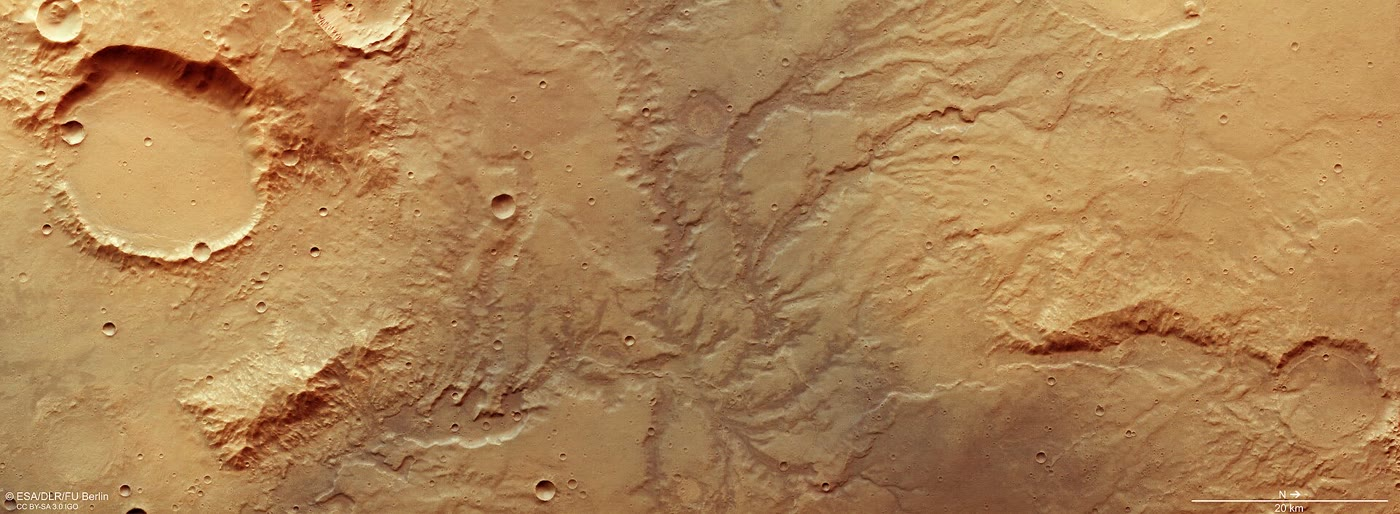
\includegraphics[width=\linewidth]{images/book5/b3-mars-valley-network.jpg}
\par\smallskip{\small मंगल पर सूखी घाटियों का एक जाल, जो मार्स एक्सप्रेस के
कैमरे से लगभग \qty{14}{m} प्रति पिक्सल पर लिया गया, \ang{17}\,S
और \ang{66}\,E के पास; उत्तर दाईं ओर है, और पैमाना-पट्टी \qty{20}{km} की है।
सहायक नदियाँ नीचे की ओर मिलकर बड़ी घाटियों में जुड़ती हैं, जो एक जल-निकास जाल का
प्रारूप है। चित्र ESA/DLR/FU Berlin, CC BY-SA 3.0 IGO के माध्यम से।}\label{fig:b3:planetary-atmospheres:valleys}
\end{omfigure}
% ledger: photo:b3-mars-valley-network

मंगल की घाटियों और प्रवाह-वाहिकाओं को भूवैज्ञानिक अनुमानों के अनुसार 100 से
\qty{1500}{m} गहरी एक वैश्विक जल-परत चाहिए, जबकि आज उसकी बर्फ़ और वायु में यह 3 से
\qty{25}{m} है। शेष का अधिकांश भाग अंतरिक्ष में चला गया। MAVEN यान ने मापा कि
सौर पवन मंगल से लगभग
\qty{100}{g} प्रति सेकंड गैस उड़ा ले जाती है, जिसका तीन-चौथाई ग्रह के पीछे की
पूँछ में, जहाँ सौर पवन बहती है, नीचे जाता है, और एक-चौथाई ध्रुवों के ऊपर
एक प्लूम में; मार्च 2015 के सौर तूफ़ानों के दौरान
हानि तेज़ हो गई, और युवा सूर्य अधिक सक्रिय था तब यह संभवतः कहीं
अधिक तेज़ थी। मंगल हाइड्रोजन भी खोता है, आज औसतन लगभग
\num{3e26} परमाणु प्रति सेकंड: चार अरब
वर्ष तक बनी रहे तो यह हानि जल की एक वैश्विक परत के बराबर होगी, जो केवल लगभग \qty{4}{m} गहरी है।
% ledger: gilli25:h-loss, lasp:maven

हानि की दर सदा आज जैसी नहीं रही है। मंगल का अक्षीय झुकाव, \ang{25.2}
अभी, पिछले 250 मिलियन वर्षों में 0 से \ang{66} के बीच डोलता रहा है,
\ang{35} के निकट के माध्य के इर्द-गिर्द, जबकि पृथ्वी का झुकाव
एक अंश से कुछ ही अधिक बदलता है। यह गति अराजक है और इसे अरबों वर्षों
पीछे तक इसका पता नहीं लगाया जा सकता; स्पर्शी संघट्टों से बने दीर्घवृत्ताकार क्रेटर,
जिनकी दिशाएँ झुकाव अभिलिखित करती हैं, वे लगभग 10 से \ang{30} के बीच का माध्य
पिछले 3.5 अरब वर्ष या उसके आसपास के दौरान सुझाते हैं। उच्च झुकाव पर ग्रीष्मकालीन ध्रुव गरम होता है,
अधिक जलवाष्प ऊपर उठता है, और जलवायु मॉडल हाइड्रोजन की हानि
बीस गुना तेज़ बताते हैं: मंगल के इतिहास भर में यह हानि जल की
लगभग \qty{80}{m} की कोटि की परत के बराबर थी।
% ledger: planet:Mars.obliq, gilli25:obliquity, holo18:obliquity, gilli25:h-loss

\section{टाइटन: मीथेन चक्र}\label{sec:b3:planetary-atmospheres:titan}

टाइटन, जो मंगल से छोटा एक चंद्रमा है, पृथ्वी से मोटा वायुमंडल रखता है:
सतही दाब लगभग 60\,\% अधिक है, \qty{-179}{\degreeCelsius} पर।
वायुमंडल लगभग 95\,\% नाइट्रोजन और 5\,\% मीथेन है, और चूँकि
चंद्रमा का गुरुत्व दुर्बल है, इसलिए वह पृथ्वी की तुलना में दस गुना ऊँचा,
लगभग \qty{600}{km} तक फैला है। ऊपरी भाग में पराबैंगनी प्रकाश मीथेन और नाइट्रोजन को तोड़ता है;
उनके टुकड़े पुनः जुड़कर भारी हाइड्रोकार्बनों की एक नारंगी धुंध बनाते हैं
जो दृश्य प्रकाश से सतह को छिपा देती है। धुंध के नीचे,
मीथेन जल की भूमिका निभाता है: वह संघनित होकर बादल बनाता है, बरसता है, नदी की वाहिकाएँ काटता है
और मीथेन तथा ईथेन की झीलें व समुद्र भरता है।
% ledger: nasa:titan-surface, nasa:titan-facts

\begin{omfigure}
\centering
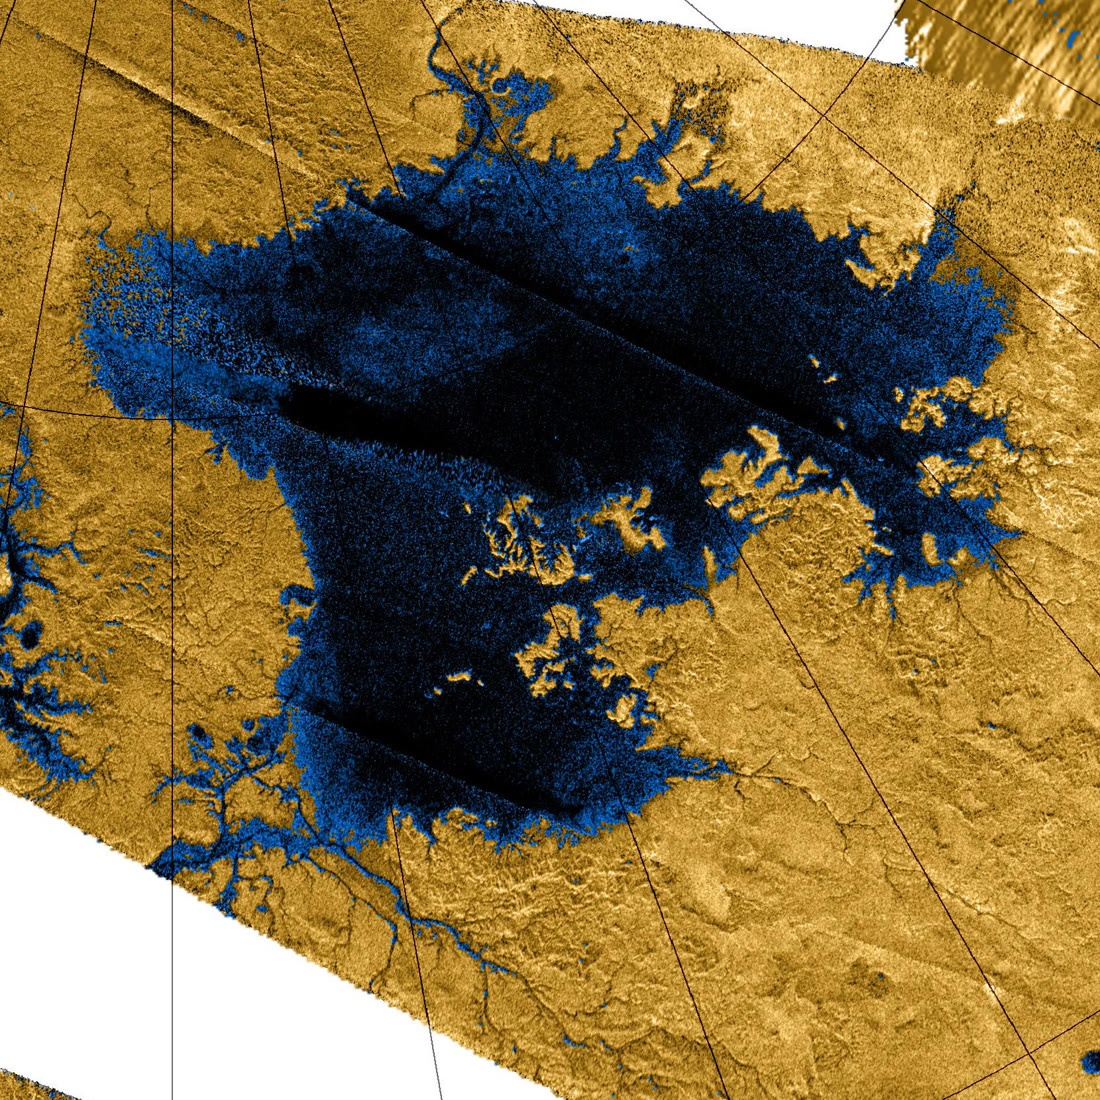
\includegraphics[width=0.5\linewidth]{images/book5/b3-ligeia-mare.jpg}
\par\smallskip{\small लिजिया मारे, टाइटन के उत्तरी ध्रुव के निकट का एक समुद्र,
कैसिनी रडार छवियों का एक मिथ्या-रंग मोज़ेक: जिन विशेषताओं को द्रव माना गया है,
नीले और काले रंग में, ठोस भूमि भूरी रंगत में, खाड़ियों और द्वीपों
और अनुमानित सहायक नदी-तंत्रों के साथ। मानचित्रित उत्तरी भाग की लगभग 400 झीलों और समुद्रों में से
जो \qty{26000}{km^2} से बड़ी हैं, वे क्षेत्र का 70\,\% धारण करती हैं।
NASA/JPL/USGS, सार्वजनिक डोमेन।}\label{fig:b3:planetary-atmospheres:ligeia}
\end{omfigure}
% ledger: photo:b3-ligeia-mare

किसी सतह पर कोई द्रव टिक सकता है या नहीं, यह उसके कला-आरेख और
वहाँ के दाब व तापमान पर निर्भर करता है। टाइटन की सतह मीथेन के
त्रिक बिंदु \qty{90.67}{K} और \qty{0.117}{bar} से ठीक ऊपर, और
उसके क्रांतिक बिंदु से नीचे है: द्रव मीथेन संभव है, और मीथेन का 5\,\% भाग
\qty{1.6}{bar} दाब पर संतृप्ति से अधिक दूर नहीं है। मंगल की सतह
जल के त्रिक बिंदु के निकट है, पृथ्वी भलीभाँति उसके द्रव क्षेत्र के भीतर है,
और शुक्र जल के क्रांतिक तापमान \qty{647}{K} से ऊपर है, जहाँ
कोई द्रव बिल्कुल नहीं टिक सकता।
% ledger: nist:methane-phase, iapws:triple-critical, nasa:titan-surface

\begin{omfigure}
\centering
\begin{tikzpicture}
\begin{axis}[width=0.8\linewidth, height=0.52\linewidth,
  xmin=60, xmax=800, ymin=1e-4, ymax=1000, ymode=log,
  xlabel={तापमान (\unit{K})}, ylabel={दाब (\unit{bar})},
  tick label style={font=\scriptsize}, label style={font=\small}]
\addplot[thick, omDef] table[x=T, y=p_bar] {figdata/out/bachelor-3-habitability-water.dat};
\addplot[thick, omDef, dashed] table[x=T, y=p_bar] {figdata/out/bachelor-3-habitability-ice.dat};
\addplot[thick, orange!80!black] table[x=T, y=p_bar] {figdata/out/bachelor-3-habitability-methane.dat};
\addplot[only marks, mark=*, mark size=1.6pt, omDef] coordinates {(273.16,0.00611657) (647.096,220.64)};
\addplot[only marks, mark=*, mark size=1.6pt, orange!80!black] coordinates {(90.67,0.1169) (190.6,46.1)};
\addplot[only marks, mark=square*, mark size=2.2pt, black] table[x=T, y=p_bar] {figdata/out/bachelor-3-habitability-bodies.dat};
\node[font=\scriptsize, anchor=south] at (axis cs:737,110) {शुक्र};
\node[font=\scriptsize, anchor=west] at (axis cs:300,1.0) {पृथ्वी};
\node[font=\scriptsize, anchor=north] at (axis cs:214,0.0045) {मंगल};
\node[font=\scriptsize, anchor=south] at (axis cs:94,2.2) {टाइटन};
\node[font=\scriptsize, omDef, anchor=west] at (axis cs:420,3) {जल: ऊपर द्रव, नीचे वाष्प};
\node[font=\scriptsize, omDef, anchor=north west] at (axis cs:205,0.0012) {बर्फ़};
\node[font=\scriptsize, orange!80!black, anchor=west] at (axis cs:196,46) {मीथेन};
\node[font=\scriptsize, omDef, anchor=south east] at (axis cs:640,230) {क्रांतिक बिंदु};
\end{axis}
\end{tikzpicture}
\par\smallskip{\small वाष्प और द्रव जल के बीच की सीमाएँ
(नीला: द्रव--वाष्प, त्रिक बिंदु से क्रांतिक बिंदु तक;
धारीदार: बर्फ़--वाष्प) और द्रव मीथेन तथा उसके वाष्प के बीच की (नारंगी),
शुक्र, पृथ्वी, मंगल और टाइटन की औसत सतही अवस्थाओं के साथ
(वर्ग)। कोई द्रव किसी सतह पर तब टिक सकता है जब वहाँ का दाब उस द्रव के वक्र से ऊपर हो,
और तापमान उसके त्रिक और
क्रांतिक तापमानों के बीच हो।}\label{fig:b3:planetary-atmospheres:phases}
\end{omfigure}
% ledger: iapws:vapour-pressure, iapws4:sublimation, iapws:triple-critical, nist:methane-phase, nasa:venus-atm, planet:Earth.Tmean, planet:Earth.psurf, nasa:mars-atm, nasa:titan-surface

टाइटन अपनी नाइट्रोजन आसानी से रोके रखता है: \omterm{def:b3:planetary-atmospheres:exobase}{बाह्य-आधार} पर नाइट्रोजन के लिए $\lambda = 41$ है,
उसका हाइड्रोजन, $\lambda$ लगभग 1.5 पर, लगभग स्वतंत्र रूप से निकल जाता है, और
आणविक हाइड्रोजन का पलायन नीचे, \omterm{def:b3:planetary-atmospheres:hydrodynamic}{होमोपॉज़} से होकर जाने वाले
सीमित फ़्लक्स से तय होता है, जैसा पृथ्वी पर होता है। टूटे मीथेन से बने भारी यौगिक
सतह पर बैठ जाते हैं, जहाँ वे विस्तृत टिब्बा-क्षेत्रों की
रेत बनाते हैं।
% ledger: gronoff:jeans-table, gronoff:diffusion, nasa:titan-surface

\section{ग्रहीय वासयोग्यता}\label{sec:b3:planetary-atmospheres:habitability}

पाठ्यपुस्तकों में बताया गया वासयोग्य क्षेत्र किसी तारे से उन दूरियों का परास है,
जिन पर पृथ्वी जैसा ग्रह अपनी
सतह पर द्रव जल बनाए रख सकता है। इसके सिरे इस अध्याय में आई सीमाएँ हैं।

\begin{definition}[ग्रहीय वासयोग्यता]\label{def:b3:planetary-atmospheres:habitability}
किसी ग्रह की \emph{ग्रहीय वासयोग्यता}\index{ग्रहीय वासयोग्यता} उसकी
भूवैज्ञानिक कालों तक अपनी सतह पर द्रव जल बनाए रखने की क्षमता है:
वह तारकीय फ़्लक्स प्राप्त करता है जो वासयोग्य क्षेत्र की सीमाओं के भीतर हो,
वह अपने वायुमंडल और जल को पलायन से बचाकर रोके रखता है,
और एक दीर्घकालिक कार्बन चक्र उसकी जलवायु को नियंत्रित करता है।
\end{definition}

वासयोग्य क्षेत्र का भीतरी किनारा आर्द्र या \omterm{def:b3:planetary-atmospheres:runaway}{अनियंत्रित
ग्रीनहाउस} है: सूर्य के चारों ओर का पृथ्वी-जैसा ग्रह \qty{0.99}{au} पर
आर्द्र हो जाता है और \qty{0.97}{au} पर अनियंत्रित हो जाता है। बाहरी किनारा
\emph{अधिकतम ग्रीनहाउस} है: कार्बन डाइऑक्साइड मिलाने से ग्रह केवल उस सीमा तक गरम होता है,
जब तक अतिरिक्त गैस अपने ग्रीनहाउस प्रभाव के लाभ से अधिक सूर्य-प्रकाश वापस बिखेरने न लगे;
सूर्य के चारों ओर यह
\qty{1.70}{au} पर होता है, लगभग \qty{8}{bar} कार्बन डाइऑक्साइड के अंतर्गत।
ये रूढ़िवादी किनारे हैं, जिनकी गणना बादलों के बिना की गई है। दो अनुभवजन्य किनारे अधिक चौड़े हैं:
शुक्र पर कम से कम एक अरब वर्षों तक सतह पर जल नहीं रहा प्रतीत होता है,
जब उसे पृथ्वी के वर्तमान सूर्य-प्रकाश का 1.76 गुना प्राप्त होता था (\qty{0.75}{au});
मंगल पर बहता जल था, जब उसे उस सूर्य-प्रकाश का 0.32 गुना प्राप्त होता था, यदि उसकी
घाटियाँ 3.8 अरब वर्ष पुरानी हैं (\qty{1.77}{au})। ठंडे तारों के चारों ओर वही सीमाएँ
कम फ़्लक्स पर आती हैं, क्योंकि उनका अधिक लाल प्रकाश
जल और कार्बन डाइऑक्साइड द्वारा कम बिखेरा और अधिक अवशोषित किया जाता है।
% ledger: kopparapu13:runaway, kopparapu13:outer, kopparapu13:hz-fit

\begin{omfigure}
\centering
\begin{tikzpicture}
\begin{axis}[width=0.8\linewidth, height=0.5\linewidth,
  xmin=0, xmax=2.1, ymin=2600, ymax=7200, x dir=reverse,
  xlabel={प्राप्त तारकीय फ़्लक्स / पृथ्वी का आज},
  ylabel={तारे का तापमान (\unit{K})},
  tick label style={font=\scriptsize}, label style={font=\small},
  legend style={font=\scriptsize, at={(0.5,-0.24)}, anchor=north, legend columns=2, draw=none}]
\addplot[name path=mg, thick, omDef] table[x=mg, y=Teff] {figdata/out/bachelor-3-habitability-hz.dat};
\addlegendentry{आर्द्र ग्रीनहाउस}
\addplot[name path=maxg, thick, red!70!black] table[x=maxg, y=Teff] {figdata/out/bachelor-3-habitability-hz.dat};
\addlegendentry{अधिकतम ग्रीनहाउस}
\addplot[thin, omDef, dashed] table[x=rg, y=Teff] {figdata/out/bachelor-3-habitability-hz.dat};
\addlegendentry{अनियंत्रित ग्रीनहाउस}
\addplot[thin, black!60, densely dotted] table[x=rv, y=Teff] {figdata/out/bachelor-3-habitability-hz.dat};
\addlegendentry{हाल का शुक्र, आरंभिक मंगल}
\addplot[thin, black!60, densely dotted, forget plot] table[x=em, y=Teff] {figdata/out/bachelor-3-habitability-hz.dat};
\addplot[green!30, opacity=0.5, forget plot] fill between[of=mg and maxg];
\addplot[only marks, mark=*, mark size=2pt, black, forget plot] coordinates {(1.911,5780) (1.0,5780) (0.431,5780)};
\node[font=\scriptsize, anchor=south] at (axis cs:1.911,5800) {शुक्र};
\node[font=\scriptsize, anchor=west, xshift=2pt] at (axis cs:1.0,5780) {पृथ्वी};
\node[font=\scriptsize, anchor=east, xshift=-2pt] at (axis cs:0.431,5780) {मंगल};
\end{axis}
\end{tikzpicture}
\par\smallskip{\small पृथ्वी जैसे ग्रह का वासयोग्य क्षेत्र, जिसे
ग्रह द्वारा प्राप्त तारकीय फ़्लक्स बनाम उसके तारे के तापमान से दर्शाया गया है (छायांकित:
\omterm{def:b3:planetary-atmospheres:runaway}{आर्द्र ग्रीनहाउस} और अधिकतम ग्रीनहाउस के बीच)। बिंदीदार: हाल के शुक्र और आरंभिक
मंगल से निकाली गई अनुभवजन्य सीमाएँ। ये फ़िट
बादल-रहित जलवायु मॉडल के हैं, जो 2600 से
\qty{7200}{K} तक वैध हैं।}\label{fig:b3:planetary-atmospheres:hz}
\end{omfigure}
% ledger: kopparapu13:hz-fit, nasa:venus, nasa:mars

केवल दूरी पर्याप्त नहीं है। ग्रह को अपना वायुमंडल थामे रखना होता है: छोटा
या गर्म ग्रह, जिसका \omterm{def:b3:planetary-atmospheres:jeans-escape}{पलायन प्राचल} कम है, अपना हाइड्रोजन खो देता है और उसके साथ
अपना जल भी, और \omterm{def:b3:planetary-atmospheres:runaway}{आर्द्र ग्रीनहाउस} में स्थित ग्रह ऊपर से सूख जाता है। ग्रह को
अरबों वर्षों तक अपनी जलवायु भी स्थिर रखनी होती है, जबकि उसका तारा
चमकीला होता जाता है: पृथ्वी पर सिलिकेट-अपक्षय तापस्थापी, जो
दीर्घकालिक कार्बन चक्र का हिस्सा है, जलवायु गर्म होने पर कार्बन डाइऑक्साइड को नीचे खींचता है
और ठंडी होने पर उसे जमा होने देता है। शुक्र पर, प्लेट विवर्तनिकी के बिना,
निर्गैसित कार्बन डाइऑक्साइड के पास चट्टानों में लौटने का कोई मार्ग नहीं रहा और वह
वायु में जमा होती गई; आज वह लगभग उतनी कार्बन डाइऑक्साइड रखता है जितनी
पृथ्वी ने कार्बोनेट चट्टानों में बंद कर रखी है। चुंबकीय क्षेत्र किसी वायुमंडल की रक्षा करता है या नहीं, यह
विवादित है: वह ऊपरी वायुमंडल को सौर पवन से बचाता है, परंतु
वह पलायन के अन्य मार्ग भी खोलता है, जैसे आयनों का
ध्रुवों के पास बहिर्वाह, और किसी ग्रह की वासयोग्यता को
केवल वासयोग्य क्षेत्र में उसके स्थान से नहीं आँका जा सकता।
% ledger: arney18:venus-loss, gronoff21:magnetic, gronoff:nonthermal

\section{अभ्यास}

\begin{exercise}[$\star$]\label{exo:b3:planetary-atmospheres:1}
शुक्र की सतह के निकट पैमाना ऊँचाई $H = RT/Mg$
(\qty{737}{K}, मोलर द्रव्यमान \qty{44.01}{g.mol^{-1}} की कार्बन डाइऑक्साइड,
$g = \qty{8.87}{m.s^{-2}}$), पृथ्वी की (\qty{288}{K},
\qty{28.97}{g.mol^{-1}}, \qty{9.80}{m.s^{-2}}), मंगल की (\qty{214}{K},
\qty{43.34}{g.mol^{-1}}, \qty{3.71}{m.s^{-2}}) और टाइटन की (\qty{94}{K},
\qty{28.0}{g.mol^{-1}}, \qty{1.35}{m.s^{-2}}) परिकलित कीजिए।
कौन-सा वायुमंडल सबसे अधिक विस्तृत है, और क्यों?
\end{exercise}

\begin{exercise}[$\star$]\label{exo:b3:planetary-atmospheres:2}
पृथ्वी का \omterm{def:b3:planetary-atmospheres:exobase}{बाह्य-आधार} \qty{500}{km} पर है (त्रिज्या \qty{6878}{km}); उसका
तापमान सौर चक्र के दौरान 800 से \qty{1600}{K} तक बदलता है। पृथ्वी का द्रव्यमान
\qty{5.97e24}{kg} मानिए। दोनों तापमानों पर हाइड्रोजन परमाणुओं का \omterm{def:b3:planetary-atmospheres:jeans-escape}{पलायन प्राचल}
तथा पलायन अंश
$(1 + \lambda)e^{-\lambda}$ परिकलित कीजिए। सौर चक्र इसे किस गुणक से बदलता है?
\end{exercise}

\begin{exercise}[$\star$]\label{exo:b3:planetary-atmospheres:3}
सूर्य के चारों ओर, पृथ्वी जैसा एक ग्रह फ़्लक्स $S_\mathrm{eff}
= 1.014$ पर आर्द्र हो जाता है, 1.0512 पर अनियंत्रित हो जाता है और 0.3438 पर अधिकतम ग्रीनहाउस तक पहुँचता है
(फ़्लक्स पृथ्वी के सापेक्ष हैं)। (क)~तीनों दूरियाँ
खगोलीय इकाइयों में परिकलित कीजिए। (ख)~शुक्र और मंगल 1.91 और 0.43
गुना पृथ्वी के सूर्य-प्रकाश को प्राप्त करते हैं। इन्हें स्थान दीजिए।
\end{exercise}

\begin{exercise}[$\star$]\label{exo:b3:planetary-atmospheres:4}
द्रव मीथेन का वाष्प दाब $\log_{10}(p/\unit{bar}) = 3.9895 -
443.028/(T/\unit{K} - 0.49)$ है। (क)~टाइटन की सतह पर,
\qty{94.15}{K} पर इसे परिकलित कीजिए। (ख)~\qty{1.6}{bar} पर मीथेन टाइटन की वायु का 5\,\% है।
इसका आंशिक दाब और सापेक्ष आर्द्रता परिकलित कीजिए। (ग)~परिणाम
टाइटन के समुद्रों से वाष्पीकरण के बारे में क्या संकेत देता है?
\end{exercise}

\begin{exercise}[$\star\star$]\label{exo:b3:planetary-atmospheres:5}
पृथ्वी के \omterm{def:b3:planetary-atmospheres:exobase}{बाह्य-आधार} पर (\qty{1000}{K}, हाइड्रोजन के लिए $\lambda = 7.02$),
ड्यूटेरियम का \omterm{def:b3:planetary-atmospheres:jeans-escape}{पलायन प्राचल}, उसकी हाइड्रोजन के सापेक्ष तापीय चाल,
और प्रति परमाणु जीन्स फ़्लक्स का अनुपात, D से H, परिकलित कीजिए। क्या \omterm{def:b3:planetary-atmospheres:jeans-escape}{जीन्स
पलायन} एक प्रबल समस्थानिक छन्ना है?
\end{exercise}

\begin{exercise}[$\star\star$]\label{exo:b3:planetary-atmospheres:6}
शुक्र के जल का D/H अनुपात \num{0.016} है; पृथ्वी के महासागरीय जल का
अनुपात \num{1.5575e-4} है। (क)~संवर्धन परिकलित कीजिए। (ख)~ड्यूटेरियम का बिल्कुल भी
पलायन न होने पर, शुक्र के जल की सबसे छोटी अतीत मात्रा क्या होगी, यदि आज वह \qty{6e15}{kg} है?
इसे ग्रह के ऊपर फैलाने पर कितनी गहराई बनेगी,
जिसका क्षेत्रफल \qty{4.60e14}{m^2} है? (ग)~जलाशय में कितनी कमी
\omterm{def:b3:planetary-atmospheres:hydrodynamic}{विसरण-सीमित पलायन}, $\alpha = 0.8$ के साथ, आवश्यक बनाएगा? निष्कर्ष निकालिए।
\end{exercise}

\begin{exercise}[$\star\star$]\label{exo:b3:planetary-atmospheres:7}
त्रिज्या \qty{3389.5}{km} वाला मंगल लगभग \num{3e26} हाइड्रोजन परमाणु
प्रति सेकंड खोता है। (क)~यदि परमाणुओं का प्रत्येक जोड़ा जल के एक अणु से आया हो, तो
चार अरब वर्षों में यह हानि जल की कितनी वैश्विक परत हटाती है?
(ख)~वही प्रश्न \num{6e27} परमाणु प्रति सेकंड पर, जो उच्च
तिर्यकता की दर है। (ग)~घाटियों और वाहिकाओं को चाहिए 100 से \qty{1500}{m} की
गहराई से तुलना कीजिए।
\end{exercise}

\begin{exercise}[$\star\star$]\label{exo:b3:planetary-atmospheres:8}
(क)~मंगल के वायुमंडल का द्रव्यमान उसके औसत पृष्ठ-दाब,
\qty{636}{Pa}, उसके गुरुत्व \qty{3.71}{m.s^{-2}} और उसकी
त्रिज्या से परिकलित कीजिए। (ख)~सौर पवन प्रति सेकंड लगभग \qty{100}{g} गैस हटाती है।
इससे चार अरब वर्षों में कितना द्रव्यमान हटेगा, और वर्तमान वायुमंडल को
कितने समय में हटा देगी? (ग)~यह अतीत की हानि का कम अनुमान क्यों है,
समझाइए।
\end{exercise}

\begin{exercise}[$\star\star$]\label{exo:b3:planetary-atmospheres:9}
बादल-रहित भाप वाले वायुमंडल वाला पृथ्वी जैसा ग्रह अपने प्राप्त सूर्य-प्रकाश का 19.3\,\%
परावर्तित करता है; उसका अवरक्त उत्सर्जन \qty{291}{W.m^{-2}} से अधिक नहीं हो सकता।
(क)~सूर्य-प्रकाश के किस फ़्लक्स से ऊपर, वाट प्रति वर्ग
मीटर में और पृथ्वी के \qty{1361}{W.m^{-2}} के सापेक्ष, यह \omterm{def:b3:planetary-atmospheres:runaway}{अनियंत्रित ग्रीनहाउस} स्थिति में चला जाता है?
(ख)~आज के शुक्र, \qty{2601}{W.m^{-2}}, और युवा शुक्र की, जो
अपनी वर्तमान दीप्ति के 70\,\% वाले सूर्य के अधीन था, तुलना कीजिए। (ग)~युवा शुक्र के लिए निष्कर्ष
अंतिम क्यों नहीं है, समझाइए।
\end{exercise}

\begin{exercise}[$\star\star\star$]\label{exo:b3:planetary-atmospheres:10}
परमाणु ऑक्सीजन का एक मॉडल तापमंडल \qty{1000}{K} पर समतापीय है, जिसमें
\qty{200}{km} पर $n = \qty{1e16}{m^{-3}}$ है; उस ऊँचाई पर $g =
\qty{9.21}{m.s^{-2}}$ और एक टक्कर-अनुप्रस्थ काट लीजिए जिसका
$\sigma_c = \qty{3e-19}{m^2}$ है। (क)~ऑक्सीजन की पैमाना ऊँचाई परिकलित कीजिए।
(ख)~\omterm{def:b3:planetary-atmospheres:exobase}{बाह्य-आधार} पर घनत्व और \omterm{def:b3:planetary-atmospheres:exobase}{बाह्य-आधार} की ऊँचाई परिकलित कीजिए।
(ग)~गुरुत्व ऊँचाई के साथ घटता है। क्या इससे \omterm{def:b3:planetary-atmospheres:exobase}{बाह्य-आधार} ऊपर
या नीचे खिसकता है?
\end{exercise}

\begin{exercise}[$\star\star\star$]\label{exo:b3:planetary-atmospheres:11}
(क)~मान लीजिए पृथ्वी का समतापमंडल आर्द्र हो गया है, जिसमें जलवाष्प का मिश्रण-अनुपात
\num{3e-3} है (जिसे $\ce{H2}$ के रूप में गिना गया है)। विसरण
सीमा $\num{3.0e13}\,f$ $\ce{H2}$ अणु प्रति वर्ग सेंटीमीटर और
प्रति सेकंड, \qty{200}{K} पर, पूरी पृथ्वी की हाइड्रोजन हानि
(त्रिज्या \qty{6371}{km}) के लिए परिकलित कीजिए। (ख)~एक महासागर,
\qty{1.4e24}{g} जल का, कितने समय तक चलेगा? पृथ्वी की आयु से तुलना कीजिए।
\end{exercise}

\begin{exercise}[$\star\star\star$]\label{exo:b3:planetary-atmospheres:12}
शुद्ध-भाप वाले ऊपरी वायुमंडल में, जो एक धूसर गैस की भाँति अवशोषित करता है, जिसमें $\kappa =
\qty{0.005}{m^2.kg^{-1}}$ है, ऐसे ग्रह पर जिसका $g = \qty{9.81}{m.s^{-2}}$
और $D = 1.66$ है: (क)~विकिरणी स्तर का दाब $p_1$ परिकलित कीजिए;
(ख)~$p_\mathrm{sat}(T) = \qty{611.657}{Pa}\,\exp[(L/R_v)(1/T_t -
1/T)]$, $L = \qty{2.5e6}{J.kg^{-1}}$, $R_v = \qty{461.5}{J.kg^{-1}.K^{-1}}$,
$T_t = \qty{273.16}{K}$ के साथ, उसका तापमान और विकिरण सीमा परिकलित कीजिए।
(ग)~रेखा-दर-रेखा सीमा \qty{291}{W.m^{-2}} है। वास्तविक जल-वाष्प का प्रभावी
$\kappa$ बड़ा होना चाहिए या छोटा?
\end{exercise}

\section{समस्या: क्या केपोस अपना जल रख पाएगा?}

\begin{problem}[{सप्ताहांत समस्या --- एक काल्पनिक
महासागर ग्रह का पलायन और ग्रहीय वासयोग्यता}]
\label{pb:b3:planetary-atmospheres:1}
केपोस एक काल्पनिक ग्रह है, जिसका द्रव्यमान \qty{5.2e24}{kg} और त्रिज्या
\qty{6200}{km} है, जिसके महासागर हैं और नाइट्रोजन तथा कार्बन
डाइऑक्साइड का वायुमंडल है। यह \qty{0.60}{au} पर एक ऐसे तारे की परिक्रमा करता है जिसकी दीप्ति
सूर्य की 0.30 गुना है और प्रभावी तापमान \qty{4800}{K} है। इसका \omterm{def:b3:planetary-atmospheres:exobase}{बाह्य-आधार}
सतह से \qty{500}{km} ऊपर, \qty{1400}{K} पर है, जिसमें
\qty{2e11}{m^{-3}} हाइड्रोजन परमाणु हैं; इसका \omterm{def:b3:planetary-atmospheres:hydrodynamic}{होमोपॉज़} \qty{200}{K} पर है,
जहाँ कार्बन डाइऑक्साइड प्रधान है और जहाँ सभी रूपों में हाइड्रोजन
मिश्रण-अनुपात $f = \num{1e-3}$ बनाता है, जिसे $\ce{H2}$ गिना गया है। एक पृथ्वी महासागर
\qty{1.4e24}{g} जल है।

\medskip\noindent\textbf{भाग I --- बाह्य-आधार।}
\begin{enumerate}
\item केपोस का पृष्ठीय गुरुत्व और माध्य घनत्व परिकलित कीजिए।
\item \omterm{def:b3:planetary-atmospheres:exobase}{बाह्य-आधार} पर पलायन वेग परिकलित कीजिए।
\item हाइड्रोजन, हीलियम और
  ऑक्सीजन परमाणुओं की तापीय चाल $u = \sqrt{2kT/m}$ \omterm{def:b3:planetary-atmospheres:exobase}{बाह्य-आधार} पर परिकलित कीजिए।
\item उनके \omterm{def:b3:planetary-atmospheres:jeans-escape}{पलायन प्राचल} परिकलित कीजिए।
\item इनमें से कौन-सा \omterm{def:b3:planetary-atmospheres:jeans-escape}{जीन्स पलायन} द्वारा महत्वपूर्ण दर से निकल सकता है?
  क्या कोई जलगतिक अवस्था के निकट है?
\item इसके तारे की सक्रिय युवावस्था के दौरान केपोस का \omterm{def:b3:planetary-atmospheres:exobase}{बाह्य-आधार} संभवतः
  \qty{3000}{K} तक पहुँच गया होगा। तब हाइड्रोजन का \omterm{def:b3:planetary-atmospheres:jeans-escape}{पलायन प्राचल} क्या था,
  और इससे क्या संकेत मिलता है?
\end{enumerate}

\medskip\noindent\textbf{भाग II --- हाइड्रोजन का जीन्स पलायन।}
\begin{enumerate}[resume]
\item हाइड्रोजन के लिए पलायन भिन्न $(1 + \lambda)e^{-\lambda}$
  परिकलित कीजिए।
\item हाइड्रोजन का जीन्स फ़्लक्स, प्रति वर्ग मीटर और प्रति सेकंड, परिकलित कीजिए।
\item पूरे \omterm{def:b3:planetary-atmospheres:exobase}{बाह्य-आधार} से निकलने वाले हाइड्रोजन परमाणुओं की
  प्रति सेकंड संख्या परिकलित कीजिए।
\item एक पृथ्वी महासागर में कितने हाइड्रोजन परमाणु हैं?
\item इस दर से केपोस को उन्हें खोने में कितना समय लगेगा?
\item ड्यूटेरियम का \omterm{def:b3:planetary-atmospheres:jeans-escape}{पलायन प्राचल} और उसकी पलायन दक्षता,
  हाइड्रोजन के सापेक्ष, प्रति परमाणु, परिकलित कीजिए।
\end{enumerate}

\medskip\noindent\textbf{भाग III --- विसरण सीमा।}
\begin{enumerate}[resume]
\item \omterm{def:b3:planetary-atmospheres:hydrodynamic}{होमोपॉज़} पर कार्बन डाइऑक्साइड की पैमाना ऊँचाई परिकलित कीजिए।
\item कार्बन डाइऑक्साइड में हाइड्रोजन का द्विआधारी विसरण प्राचल
  \qty{200}{K} पर $b = \qty{1.2e19}{cm^{-1}.s^{-1}}$ है। हाइड्रोजन का
  $\ce{H2}$ का विसरण-सीमित फ़्लक्स, प्रति वर्ग मीटर और प्रति सेकंड, परिकलित कीजिए।
\item पृथ्वी की सीमा $\num{3.0e13}\,f$ अणु प्रति
  वर्ग सेंटीमीटर और प्रति सेकंड वाली सीमा से तुलना करके इसकी जाँच कीजिए, गुरुत्व के अनुपात में समायोजित करके।
\item विसरण सीमा द्वारा पूरे ग्रह के ऊपरी वायुमंडल को प्रति सेकंड मिल सकने वाले हाइड्रोजन परमाणुओं की
  संख्या परिकलित कीजिए (पृष्ठ का क्षेत्रफल
  लीजिए)।
\item प्रश्न~9 से तुलना कीजिए। कौन-सी प्रक्रिया पलायन को सीमित करती है, और
  तापमंडल के हाइड्रोजन का क्या होता है?
\item \omterm{def:b3:planetary-atmospheres:exobase}{बाह्य-आधार} पर हाइड्रोजन का कौन-सा घनत्व होगा, जिससे \omterm{def:b3:planetary-atmospheres:jeans-escape}{जीन्स पलायन}
  संपूर्ण आपूर्ति का वहन कर सके?
\item विसरण सीमा पर केपोस को हाइड्रोजन का एक पृथ्वी महासागर
  खोने में कितना समय लगेगा?
\end{enumerate}

\medskip\noindent\textbf{भाग IV --- क्या केपोस वासयोग्य क्षेत्र में है?}
\begin{enumerate}[resume]
\item केपोस को मिलने वाला तारकीय फ़्लक्स, पृथ्वी के सापेक्ष, परिकलित कीजिए।
\item \qty{4800}{K} के तारे के लिए \omterm{def:b3:planetary-atmospheres:runaway}{आर्द्र ग्रीनहाउस} सीमा
  $S_\mathrm{eff} = 0.939$ पर है और अधिकतम ग्रीनहाउस 0.290 पर। वासयोग्य क्षेत्र की
  सीमाएँ खगोलीय इकाइयों में परिकलित कीजिए और केपोस को स्थित कीजिए।
\item केपोस के आंतरिक किनारे तक पहुँचने से पहले तारे को किस गुणक से
  दीप्त होना होगा?
\item 0.3 के एल्बिडो पर केपोस द्वारा प्रति वर्ग
  मीटर अवशोषित सूर्य-प्रकाश और उसका साम्य तापमान परिकलित कीजिए। इसकी
  \omterm{def:b3:planetary-atmospheres:runaway}{अनियंत्रित ग्रीनहाउस सीमा} से तुलना कीजिए।
\item यदि एक गर्म जलवायु ने केपोस के समतापमंडल को आर्द्र बना दिया हो,
  जिसमें $f = \num{3e-3}$ हो, तो एक पृथ्वी महासागर कितने समय तक चलेगा?
\item \omterm{def:b3:planetary-atmospheres:hydrodynamic}{विसरण-सीमित पलायन} द्वारा केपोस को हाइड्रोजन का एक पृथ्वी महासागर
  $f = \num{1e-3}$ के साथ खोने में लगने वाला समय, अरब वर्षों में, दो
  सार्थक अंकों तक दीजिए।
\end{enumerate}
\end{problem}
% ledger: zahnle19:diffusion, kopparapu13:hz-fit, kopparapu13:runaway, gronoff:jeans, const:G, const:kB, const:NA
